\chapter{Un transmisor ISDBT implementado en GNU Radio}

\section{Generalidades del Transmisor}
Por ejemplo algunas
\section{El flujo de datos en GNU Radio}

Para el desarrollo de los bloques de gr-isdbt-tx, fue necesario comprender el modo en el que los datos se mueven entre bloques en GNU Radio. El motor del programa realiza llamados de forma periódica a los bloques en el flowgraph, dependiendo de la cantidad de muestras que tenga en cola para procesar en cada bloque, y de la tasa de muestras que busque mantener constante a traves del sistema, le comunica a cada bloque, la cantidad de datos que necesita que le dejen en salida.  

Al momento de crear un nuevo bloque, debemos especificar en la firma de la función, los parámetros necesarios para que el motor central pueda controlar de flujo de datos de nuestro nuevo bloque. Para realizar esto, se utilizan ciertos parámetros, precargados en la estructura de clases de los bloques, orientados a la entrada/salida de datos, estos son,  noutputitems y ninputitems. 

Mediante estas variables, el motor de procesamiento puede obligar a los bloques a ejecutarse mas de una vez en cada llamado, pues exige la cantidad de salidas que necesita para mantener la tasa. Para esto, le notifica al bloque en la variable noutputitems, la cantidad de “tandas” de datos que la instancia actual del bloque necesita devolverle al motor de procesamiento para mantener la tasa. 

La variable ninputitems, mantiene el control de la cantidad de datos que hay en cada uno de los puertos de entrada. Y utilizándola como variable, podemos especificar cuantos datos de entrada precisamos consumir para obtener un dato en el puerto de salida.

Esta operación depende bastante de la naturaleza del bloque, por ejemplo, en los bloques síncronos, se sabe de antemano que la tasa de muestras se mantendrá constante, por lo que alcanza con especificar el tipo y la cantidad de muestras que atravesaran el bloque en una ejecución. 

Los bloques de tipo general, son mas complicados, pues es necesario especificar explícitamente la relación entre la cantidad de muestras a la entrada y a la salida. Este control de flujo se realiza desde un método, precargado en la clase con la que se crea el bloque, denominado forecast.

\section{Obtencion de los TSP por capa}

Como se explico anteriormente, en un solo flujo de transporte coexisten paquetes pertenecientes a las distintas capas de transmisión, sino que también están las tablas de información, y los paquetes nulos para mantener el flujo de datos constante. 

Es necesario separar al principio del transmisor, esta información, para procesarla individualmente cada capa, afín de lograr mantener los programas contenidos en la misma en un mismo flujo, pues como vimos, las capas pueden tener distintas modulaciones y distintos retardos. 

Cada paquete tiene en su encabezado IIP, un parametro denominado \textit{layer\_information}, que contiene información sobre la capa de transporte a la que pertenece. El parametro ocupa los primeros cuatro bits del segundo byte del encabezado del TSP, y se decodifica según la siguiente tabla

\begin{table}[h!]
	\centering
	\begin{tabular}{|c|c|}
		\hline
		\textbf{Valor $b_{7}b_{6}b_{5}b_{4}$} & \textbf{Capa}\\
		\hline
		0000 		& Null TSP\\
		\hline
		0001 		& Capa A\\
		\hline
		0010 		& Capa B\\
		\hline
		0011 		& Capa C\\
		\hline
	\end{tabular}
	\caption{\label{Identificador de capa para TSP} Par\'ametro indicador de capa en el IIP.}
\end{table}

El primero de los bloques de gr-isdbt-tx, es un bloque que se encarga de realizar esta tarea. Dado que conocemos de antemano la cantidad de TSPs que estan contendios en un cuadro multiplex de nuestro BTS de prueba, definimos un bloque con un puerto de entrada y tres puertos de salida. En cada ejecucion, se recorre un cuadro multiplex, analizando para cada uno de los TSP el parámetro \textit{layer\_information}, decodificamos a que capa pertenece, y se enrutan según corresponda. 

Entendemos que la implementación que presentamos de este bloque, existen cosas a mejorar. No las incluimos en este release del código por cuestiones de tiempo. De primera mano, la cantidad de TSP por cuadro multiplex podría ser calculada en tiempo de ejecución, para el BTS que el usuario quiera usar en ese momento, al igual que la cantidad de paquetes de cada capa. Hoy esos parámetros están fijados, y eso limita la robustez del transmisor. Discutiremos estos temas mas a fondo en el capitulo 7.

\section{Codificaciones de Canal}

	\subsection{Reed Solomon}
La norma ISDBT utiliza una implementación exactamente similar a la de DVB-T del codificador Reed Solomon. En cada TSP se sustituyen los últimos 16 bytes del IIP por la palabra de redundancia de un codigo RS(204,188). Para lograr esta distancia, lo que se hace es llevar el payload hacia un tamaño mas grande, agregando 51 bytes en 0 al comienzo del TSP. Luego, el nuevo payload de 239 bytes, se inyecta en un codificador RS(255,239). 

El cambio de tamaño se realiza principalmente para utilizar un algoritmo mas eficiente. Una vez obtenida la palabra codigo del mismo, se remueven los primeros 51 bytes nulos, y obtenemos el codigo RS(204,188) que entra en el tamaño de un TSP, y ademas es capaz de corregir errores hasta de 8 bytes. 

Para la implementacion de esta funcionalidad en ISDB-T, no fue necesario desarrollar ningun bloque. Dentro de los complementos de GNU Radio esta el paquete gr-dvb \cite{gr-dvb} (originalmente un proyecto de terceros, que en 2015 fue incorporado al repositorio oficial de GNU Radio), que contiene los bloques necesarios para implementar tanto un transmisor como un receptor bajo la norma DVB. Al compartir el codificador Reed Solomon con ISDBT, basto con utilizar el bloque de gr-dvb.

\begin{figure}[h!]
	\centering
	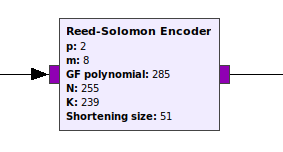
\includegraphics[scale=0.5]{figuras/cap05/RSencoder}
	\caption{\label{f:RSencoder} Bloque Reed Solomon Encoder de gr-dvb.}
\end{figure}

En la figura 5.1, mostramos el bloque y la configuracion parametrica del mismo, tal cual se implemento en gr-isdbt-tx. Los parametros \textbf{p}, \textbf{m} y \textbf{GF polynomial} son los que configuran el polinomio generador que es la base del algoritmo. Para lograr el polinomio generador del algoritmo para RS(255,239), debemos utilizar el polinomio:

\begin{gather*}
	p(x) = x^8 + x^4 + x^3 + x^2 + 1
\end{gather*}

	\subsection{Viterbi}
	Otro de los códigos de canal implementados por ISDBT es el código Viterbi. Este código, es  convolucional con puncturing, su codigo madre tiene una tasa de $\frac{1}{2}$ y constante $k = 7$, lo que permite obtener en salida datos codificados a cualquier tasa m/n en transmisión, sin aumentar la complejidad de la decodificación en recepción. 
	
	Esto sucede, porque tanto el lado transmisor como el receptor, conocen la llamada matriz de puncturing. En esa matriz, se especifica para cada tasa de código buscadas, los bits redundantes que serán eliminados al transmitir, para lograr la tasa deseada. Vale recordar que estos bits deben ser reingresados por el decodificador en recepción, pues de lo contrario aumentaría fuertemente la complejidad de la decodificación.
	
	\begin{figure}[h!]
		\centering
		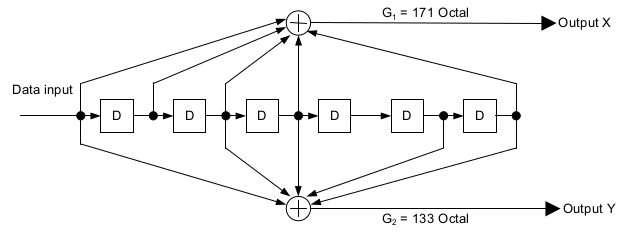
\includegraphics[scale=0.5]{figuras/cap05/viterbi}
		\caption{\label{f:viterbi} Circuito del codigo madre del Viterbi que implementa ISDBT.}
	\end{figure}
	
	Agregar este tipo de códigos a la cadena de transmisión, aumenta la resistencia ante las perdidas y mantiene una tasa de bits constante, lo que colabora con el mantenimiento del sincronismo del sistema.
	
	DVB utiliza el mismo código en su cadena de transmisión, con los mismos parámetros, por lo que en gr-isdbt-tx, no fue necesario realizar un desarrollo del bloque sino que reutilizamos el existente en gr-dvb. 
	
	\begin{figure}[h!]
		\centering
		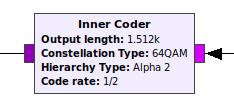
\includegraphics[scale=0.5]{figuras/cap05/inner}
		\caption{\label{f:inner} Bloque de gr-dvb que implementa el codificador Viterbi.}
	\end{figure}
	
\section{La modulacion}

Para resolver la modulación en nuestro transmisor, decidimos crear un solo bloque que resuelva en conjunto los problemas de interleaving de bits y modulacion. Esto resulto bastante conveniente, pues basto con crear una variable que contenga un selector de modulacion, y en base a el se crean una serie de colas, cuyos tamaños responden a lo explicado sobre interleaving en el inciso 5.7.

\begin{figure}[h!]
	\centering
	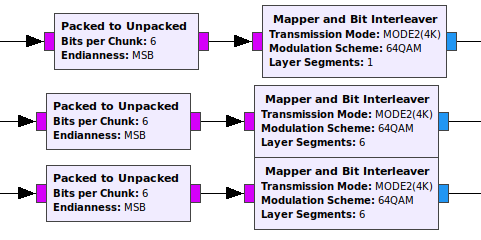
\includegraphics[scale=0.5]{figuras/cap05/modulacion}
	\caption{\label{f:modulacion} Implementacion de la modulacion e interleaving a nivel de bits en gr-isdbt-tx.}
\end{figure}


El problema que nos encontramos en esta etapa, fue el de particionar la informacion en un byte, pero conservar el resto. Un ejemplo claro de esto se da cuando la modulacion es \textit{64-QAM}, pues cada simbolo en este caso se construye con 6 bits. Ahora, el parseo de datos entre bloques, GNU Radio lo hace encapsulados en datos de tipo \textit{byte}. Por lo tanto, necesitabamos una forma de resolver el problema de separar 6 bits utiles de un dato, y guardar los 2 siguientes para el proximo simbolo. En principio, no pareceria ser un problema tan grave, pero podria pasar que los 2 bits que nos quedan pendientes, se correspondan con un simbolo que se construira en una proxima llamada al metodo modulador del objeto "bloque mapper". A nivel de programacion, esto implica que la memoria volatil de la instancia del objeto, se borra, por lo que habria que utilizar algun almacenamiento que permanezca en memoria estatica, y actualizarla en cada simbolo que se procesa.

Recorrer ese camino nos pareció ademas de muy laborioso, poco eficiente en terminos de CPU. Encontramos la solucion en un conjunto de bloques propietarios de GNU Radio, que lo resuelven de manera eficiente. Los bloques \textit{Packed to Unpacked} nos resuelven el problema. Basta con tener en cuenta a la hora de utilizar el tranmisor, definirle el parametro de \textit{Bits per Chunk} de forma consistente con la modulacion que se este utilizando. 

\begin{table}[h!]
	\centering
	\begin{tabular}{|c|c|}
		\hline
		\textbf{Modulación} & \textbf{Bits por símbolo}\\
		\hline
		QPSK		& 2\\
		\hline
		16-QAM 		& 4\\
		\hline
		64-QAM		& 6\\
		\hline
	\end{tabular}
	\caption{\label{Bits por simbolo segun modulacion} Bits por símbolo según modulación.}
\end{table}

A la salida de los bloques \textit{Bits per Chunk}, tendremos un byte completo de 8 bits, pero rellenado con la cantidad de bits requerida por la modulación, comenzando por el bit mas significativo.  Esto nos permite normalizar la recepción de datos del bloque modulador, para cada caso, sabremos perfectamente como esta compuesto el byte de datos. 

Una vez allí, alcanza con crear una cola con el retardo correspondiente, y enrutar los bits hacia la misma de forma ordenada. La secciona de modulación del bloque, funciona de la siguiente manera. 

Se obtiene de la cola los bits a procesar, y se arma, manteniendo el orden especificado en la norma, una palabra de N bits, donde $N={2,4,6}$ según corresponda en la tabla \tablename{Bits por simbolo segun modulacion}. Una vez formada la palabra, se re interpreta como un numero decimal, y se busca en un arreglo el complejo que se corresponda con la palabra recién formada. Esta información se obtiene de la tabla   

\section{El uso de los entrelazamientos}
\section{Formacion de cuadros OFDM}
	\subsection{Las portadoras piloto}
	\subsection{Las portadoras activas}
\section{El prefijo ciclico}
\section{La transmision desde USRP}